\documentclass[13pt,a4paper]{article}
\usepackage{a4wide,amssymb,epsfig,latexsym,multicol,array,hhline,fancyhdr}
\usepackage{amsmath}
\usepackage{amsfonts}
\usepackage{lastpage}
\usepackage[lined,boxed,commentsnumbered]{algorithm2e}
\usepackage{algpseudocode}
\usepackage{enumerate}
\usepackage{color}
\usepackage{graphicx}							% Standard graphics package
\usepackage{array}
\usepackage{tabularx, caption}
\usepackage{multirow}
\usepackage{multicol}
\usepackage{rotating}
\usepackage{graphics}
\usepackage{geometry}
\usepackage{setspace}
\usepackage{subfig}
\usepackage{epsfig}
\usepackage{tikz}
\usepackage{esvect}
\usepackage{subcaption}
\usepackage{listings}
\usepackage{mathtools}
\usepackage{subcaption}
\usepackage[
sorting=none, 
backend=biber,
style=alphabetic,
]{biblatex}
\addbibresource{reference.bib}
\usetikzlibrary{arrows,snakes,backgrounds}
\usepackage{hyperref}
\hypersetup{urlcolor=blue,linkcolor=black,citecolor=black,colorlinks=true} 
%\usepackage{pstcol} 								% PSTricks with the standard color package

\newtheorem{theorem}{{\bf Theorem}}
\newtheorem{property}{{\bf Property}}
\newtheorem{proposition}{{\bf Proposition}}
\newtheorem{corollary}[proposition]{{\bf Corollary}}
\newtheorem{lemma}[proposition]{{\bf Lemma}}


% Default fixed font does not support bold face
\DeclareFixedFont{\ttb}{T1}{txtt}{bx}{n}{12} % for bold
\DeclareFixedFont{\ttm}{T1}{txtt}{m}{n}{10}  % for normal


% Custom colors
\usepackage{color}
\definecolor{deepblue}{rgb}{0,0,0.5}
\definecolor{deepred}{rgb}{0.6,0,0}
\definecolor{deepgreen}{rgb}{0,0.5,0}

\usepackage{listings}

% Python style for highlighting
\newcommand\pythonstyle{\lstset{
		language=Python,
		basicstyle=\ttm,
		morekeywords={self},              % Add keywords here
		keywordstyle=\ttb\color{deepblue},
		emph={MyClass,__init__},          % Custom highlighting
		emphstyle=\ttb\color{deepred},    % Custom highlighting style
		stringstyle=\color{deepgreen},
		frame=tb,                         % Any extra options here
		showstringspaces=false
}}


% Python environment
\lstnewenvironment{python}[1][]
{
	\pythonstyle
	\lstset{#1}
}
{}

% Python for external files
\newcommand\pythonexternal[2][]{{
		\pythonstyle
		\lstinputlisting[#1]{#2}}}

% Python for inline
\newcommand\pythoninline[1]{{\pythonstyle\lstinline!#1!}}

\AtBeginDocument{\renewcommand*\contentsname{Table of Contents}}
\AtBeginDocument{\renewcommand*\refname{References}}
%%%
\setcounter{secnumdepth}{4}
\setcounter{tocdepth}{3}
\makeatletter
\newcounter {subsubsubsection}[subsubsection]
\renewcommand\thesubsubsubsection{\thesubsubsection .\@alph\c@subsubsubsection}
\newcommand\subsubsubsection{\@startsection{subsubsubsection}{4}{\z@}%
	{-3.25ex\@plus -1ex \@minus -.2ex}%
	{1.5ex \@plus .2ex}%
	{\normalfont\normalsize\bfseries}}
\newcommand*\l@subsubsubsection{\@dottedtocline{3}{10.0em}{4.1em}}
\newcommand*{\subsubsubsectionmark}[1]{}
\renewcommand\listoffigures{%
	\section*{\listfigurename}%
	\@mkboth{\MakeUppercase\listfigurename}%
	{\MakeUppercase\listfigurename}%
	\@starttoc{lof}%
}
\makeatother

\begin{document}
	\section{ABC}	
	abc
	\newpage
	
	\subsection{Robot Global Vision Update}
		\subsubsection{Introduction}
		Robot Global Vision Update is a component of Autonomous Robot system. This component is designed and implemented in python programming language, with missions determining open sights and identifying open points based on the map figure from the SLAM node (belonging to the Robot System component). After determining the best open point to go to, this component analyses and publish a message that is a sequence of points the robot has to go through to get to the next point.
		\subsubsection{Role}
		In essence, in the Autonomous Robot system, Robot Global Vision Update has the role of identifying and storing information from around environment, thereby making decisions about the next points that the robot needs to go to. \\
		Specifically, after Robot Global Vision Update has been started, it will go through the following works below:
		\begin{itemize}
			\item Receive two values "x" and "y" from users that are used to represent the actual coordinates of the Goal.
			\item The goal coordinates will undergo a mapping step from the real coordinates (fixed) to the robot's relative coordinates (set when the ROS Bringup node starts). The mapping step is implemented in the Paper Finder component.
			\item After receiving the goal coordinates that have been mapped, this component begins to analyse and send the set of points, including the current coordinates and the coordinates of points that need to be traversed, to the Robot Motion Node component.
			\item After receiving the done moving message from Robot Motion Node, this Node will continue to calculate and return the next point to go. This process repeats until the robot reaches its goal.
		\end{itemize}
		
		\subsubsection{Published - subscribed topics}
		Because Autonomous Robot system uses on a publisher-subscriber protocol, the Robot Global Vision Update is a node of the system, whith sends and receives messages between the nodes through publishing and subscribing to a specific topics.
		\begin{figure}[!h]
			\centering
			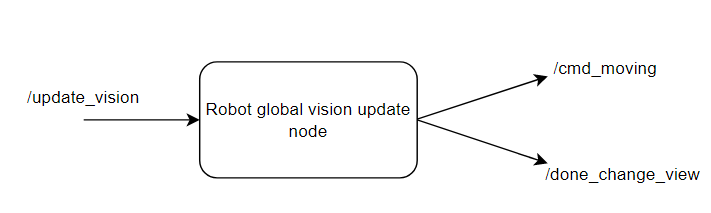
\includegraphics[width=1\textwidth]{Robot_Global_Vision_Update/RGVU_node_pub_sub.png}
			\caption{Topics are published or subscribed by Robot Global Vision Update}
		\end{figure} \\ \\ \\
		About topics which registered to publish:
		\begin{itemize}
			\item /done\_change\_view: is the topic used to publishing/subscribing requests to recognize the actual coordinates from objects on the camera view. After Robot Global Vision Update initialized, it will send to this topic the goal coordinates entered by the user with the format "[\{x coordinate\}, \{y coordinate\}]".
			\item /cmd\_moving: is the topic used to publishing/subscribing messages which is a set of points to move to. After determining the next point to go to, Robot Global Vision Update will send a message to this topic which has the format is a set of points with the first point being the current coordinates of the robot and the remaining points being the points that the robot has to go through.
		\end{itemize}
		About topics that have been registered for subscription:
		\begin{itemize}
			\item /update\_vision: is the topic used to publishing/subscribing a message containing the coordinates of a mapped destination or a confirmation message that notices the robot moved to the next point. Robot Global Vision Update subscribes to this topic to receive information about the mapped destination coordinates and passed a message to start the calculation and return the next set of points to go to.
		\end{itemize}
		
		\subsubsection{Flow chart}
		abc
		\subsubsection{State machine}
		abc
		\subsubsection{Algorithms are applied}
		Since the Autonomous Robot system applies the method of moving according to the sets of points in unknown environment, it is very important to prioritize choosing safe open points. The open points must ensure the safety of the robot during and after moving. In addition, the travel distance must be optimized to save the robot's power energy. \\
		Therefore, Robot Global Vision Update component applied algorithms to process data, involved in:
		\begin{itemize}
			\item Processing obstacles taken from SLAM map through Canny algorithm.
			\item Determining open sights and local open points at the current position of the Robot.
			\item Saving open points to visibility graph and reconstruct graph.
			\item Find next point to go to and approximately path to go to next point with has optimal distance.
			\item Remove the non-optimal points inside approximately path.
		\end{itemize}
			\paragraph{Processing obstacles taken from SLAM map through Canny algorithm\\}
			SLAM map is the image returned after the SLAM algorithm processes the data scanned by Lidar. We used Canny algorithm to analyse SLAM map and it return a list of obstacles, which are represented by a list of points that are the coordinates of the obstacle's vertices. \\
			The algorithm determines the open area based on the obstacles inside robot vision (has value between $120mm - 3,500mm$, default is $1,000mm$). However, obstacles taken from the SLAM map is not a true polygon in the geometry theory, it has noisy vertices that form redundant edges, which affects the algorithm to enlarge the obstacles (Described in detail below).
			\begin{figure}[!h]
				\centering
				
\includegraphics[width=0.7\textwidth]{Robot_Global_Vision_Update/RGVU_original_obstacle.png}
				\caption{Obstacle which has redundant edges}
			\end{figure} \\
			Regarding the concept of an obstacles represented by a set of points, we convention that all obstacles applied in the program are polygon satisfying the following three conditions:
			\begin{itemize}
				\item There is no three collinear vertices lying on the same line. Experimentally, we saw that there are four possible cases of three collinear vertices.
				\begin{figure}[!h]
					\centering
					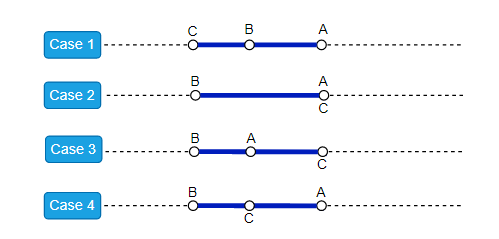
\includegraphics[width=0.7\textwidth]{Robot_Global_Vision_Update/RGVU_4case_thanghang.png}
					\caption{Four cases that 3 collinear vertices in order A$\rightarrow$B$\rightarrow$C}
				\end{figure}
				
				\item There is no two sides cross each other. Experimentally, we find that this condition is always true for the obstacles after being processed by Canny algorithm.
				\item The obstacle is a polygon with no internal holes. This condition means that in a set of points of the obstacle, the begin and the end points always coincide.\\
				\begin{figure}
					\centering
					\subfloat[\centering Obstacle is not true polygon]{{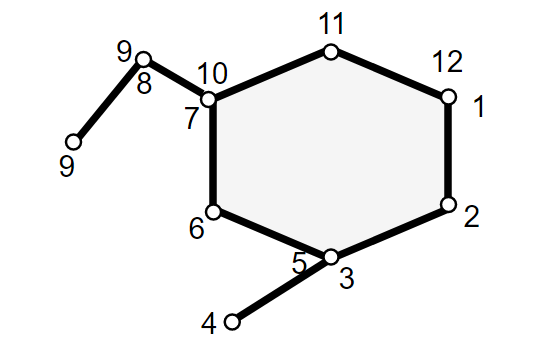
\includegraphics[width=6cm]{Robot_Global_Vision_Update/RVGU_false_ob.png} }}%
					\qquad
					\subfloat[\centering Obstacle is true polygon]{{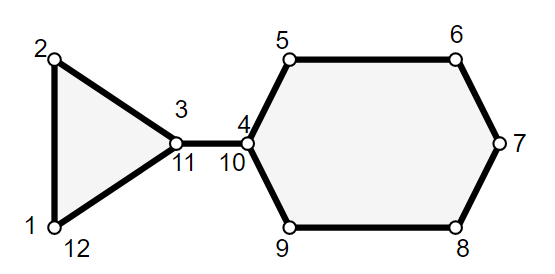
\includegraphics[width=6cm]{Robot_Global_Vision_Update/RVGU_true_ob.png} }}%
					\caption{List of obstacle with vertex numbers as the index in list}
					\label{fig:my_label}
				\end{figure}
			\end{itemize}
			
			Based on the conventions about obstacles that described above, we need to pre-process obstacles data before applying the obstacle zoom in algorithm. The algorithm which we implemented for obstacles pre-processing step named \textit{Three collinear adjacent vertices removing}.
			
			\begin{itemize}
				\item[$\ast$] \textbf{Three collinear adjacent vertices removing algorithm}\\
				\textit{Three collinear adjacent vertices removing} algorithm is implemented to reconstruct obstacles data whenever it found three collinear adjacent vertices in the obstacle.\\
				In the first condition of an accurate polygon as described above, we clarified that if an obstacle is an accurate polygon, there are no three collinear adjacent vertices in the obstacle. That is why we need to implement and apply this algorithm to the Robot Global Vision Update component.\\
				In \textit{Three collinear adjacent vertices removing} algorithm, we compare the length of three line segments formed by pair of two vertices in three adjacent vertices. If there exists a line segment that is equal to the sum of the other two line segments, then they are collinear. Based on two vertices which are the two ends of the longest line segment, we know the order of the three vertices and the vertex are between 2 other vertices. Since we consider every 3 vertices in a time, there are 4 cases as described in Figure \{...\}. However, We minimize to 3 cases because case 1 and case 2 of figure A have the same treatment in this algorithm.\\
				For example, if we assign current vertex is \textit{B}, previous vertex is \textit{A} and after vertex is \textit{C}, by comparing the lenght of \textit{AB}, \textit{BC} and \textit{AC}, we know that there 3 cases:
				\begin{itemize}
					\item If $AB + BC = AC$, then B is between A and C. In this case, the algorithm will pop B out of vertices list of the obstacle. \\
					\begin{figure}[!h]
						\centering                                 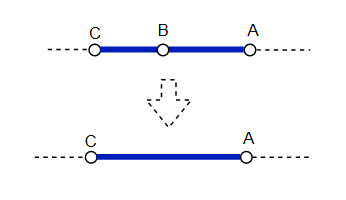
\includegraphics[width=0.7\textwidth]{Robot_Global_Vision_Update/RGVU_preprocess_case1.png}
						\caption{Case 1 solved by the algorithm in order A$\rightarrow$B$\rightarrow$C}
					\end{figure} \\
					After processing, the list of vertices will change from $[..., A, B, C, ...]$ to $[..., A, C, ...]$.
					\item If $AC + BC = AB$, then C is between A and B or C duplicates with A. In this case, the algorithm will add new vertex named B' such that BB' is perpendicular to AB and the length of BB' is equal to $\gamma$ which is very small (fixed value). \\
					\begin{figure}[!h]
						\centering                                 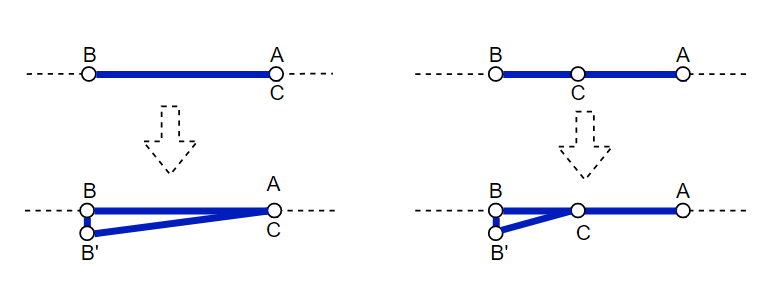
\includegraphics[width=0.7\textwidth]{Robot_Global_Vision_Update/RGVU_preprocess_case2.png}
						\caption{Case 2 solved by the algorithm in order A$\rightarrow$B$\rightarrow$C}
					\end{figure} \\
					After processing, the list of vertices will change from $[..., A, B, C, ...]$ to $[..., A, B, B', C, ...]$.
					\item If $AB + AC = BC$, then A is between B and C. In this case, the algorithm will add two new vertices named B' and A'. B' is the same as described in case 2 and A' is the same as A.\\
					\begin{figure}[!h]
						\centering                                 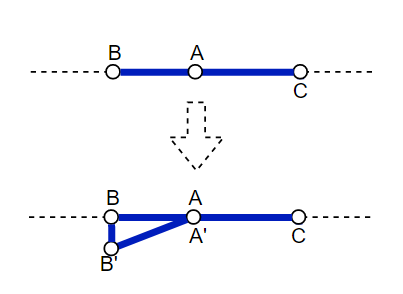
\includegraphics[width=0.7\textwidth]{Robot_Global_Vision_Update/RGVU_preprocess_case3.png}
						\caption{Case 3 solved by the algorithm in order A$\rightarrow$B$\rightarrow$C}
					\end{figure} \\
					After processing, the list of vertices will change from $[..., A, B, C, ...]$ to $[..., A, B, B', A', C, ...]$.
					\item Otherwise, three adjacent vertices that are being considered, is not collinear.
				\end{itemize}
				In reality, three collinear adjacent vertices usually noisy signals when slam gets data from lidar. However, we implemented the algorithm to handle this case without discarding them. If we choose the way that removes the collinear adjacent vertices, there is a risk that the obstacle may be changed from reality, which affects the safety of the robot during movement. Instead, we add or remove vertices without changing the original structure. This way means that accepting noisy data is also an obstacle, but this noise data usually be outside the robot's vision, so we don't need to care about them. \\
				\begin{figure}[!h]
					\centering                                 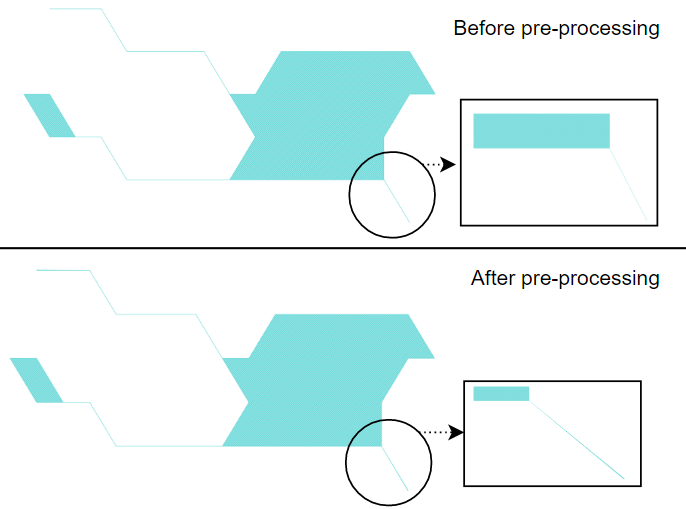
\includegraphics[width=0.7\textwidth]{Robot_Global_Vision_Update/RGVU_preprocess_result.png}
					\caption{Obstacle before and after pre-processing step}
				\end{figure} \\
				\item[$\ast$] \textbf{Obstacles zooming-in algorithm} \\
				The \textit{Obstacles zooming-in} algorithm is the algorithm that zooms-in obstacles by value of robot radius (fixed value, default is $115mm$).\\
				The Autonomous Robot system is constructed by path-planning method, which means the robot moves point by point in the set of points processed by the Robot Global Vision Update component. In the open sights and open points finding algorithm (described below), open sights is determined by checking vertices of obstacles inside robot's vision. Therefore, if we don't zoom-in obstacles before finding open sights and open points, the algorithm can determine an open point that is too close to the obstacle. This happens because the algorithm only considers the robot as a point, despite in fact the robot is a block with a radius greater than 0. For this reason, the application of \textit{Obstacles zooming-in} algorithm is necessary to ensure the selection of an open points, so that the robot will be safe to move to that points.\\
				For each edge of an obstacle, the algorithm finds normal vector and move the vertices in the direction of the vector found. The algorithm is always sure that that new obstacle cover old obstacle and all points on the polygon after zooming will be at a distance to old polygon greater than or equal to the robot radius. \\
				In detail, The algorithm consists of these step:
				\begin{itemize}
					\item Check if the normal vector direction is out of the obstacle.
					\begin{figure}[!h]
						\centering                                 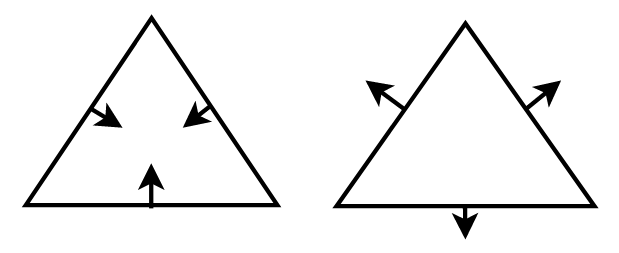
\includegraphics[width=0.7\textwidth]{Robot_Global_Vision_Update/RGVU_fconfig_lefthand.png}
						\caption{Normal vectors direction inside (left) and outside (rignt) of obstacle}
					\end{figure} \\
					We created an algorithm to check if the normal vector direction is out of the obstacle, that is named left hand direction algorithm. \\
					The left hand direction algorithm is implemented based on the \textit{Jordan Curve Theorem}. It says that "a point is inside a polygon if, for any ray from this point, there is an odd number of crossings of the ray with the polygon's edges". In the left hand direction algorithm, we find a point based on the normal vector of an edge of the obstacle, then we choose any ray peeking out from the selected point and check its number of intersection points with the obstacle. If intersection points is odd, which means current normal vector direction is inside ob the obstacle, the left hand direction algorithm will return False. Otherwise, it return True.\\
					\begin{figure}[!h]
						\centering                                 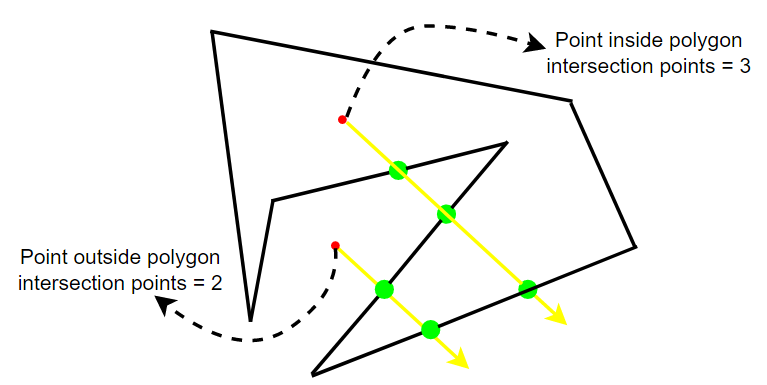
\includegraphics[width=0.7\textwidth]{Robot_Global_Vision_Update/RGVU_fconfig_lefthand_1.png}
						\caption{Jordan Curve Theorem}
					\end{figure} \\
					
					\item After got the corrent direction of normal vector, the algorithm will traverse each pair of adjacent edges of the obstacle. In this step, there are two cases that need to be process:
					\begin{itemize}
						\item[$\circ$] If two edges form a concave vertex, then the algorithm will find normal vectors for 2 edges, then move the two edges in the direction of the normal vector. Finally, the algorithm calculates the intersection point of two edges after moving and updating the new vertex is the intersection of those two edges. \\
						\begin{figure}[!h]
							\centering                                 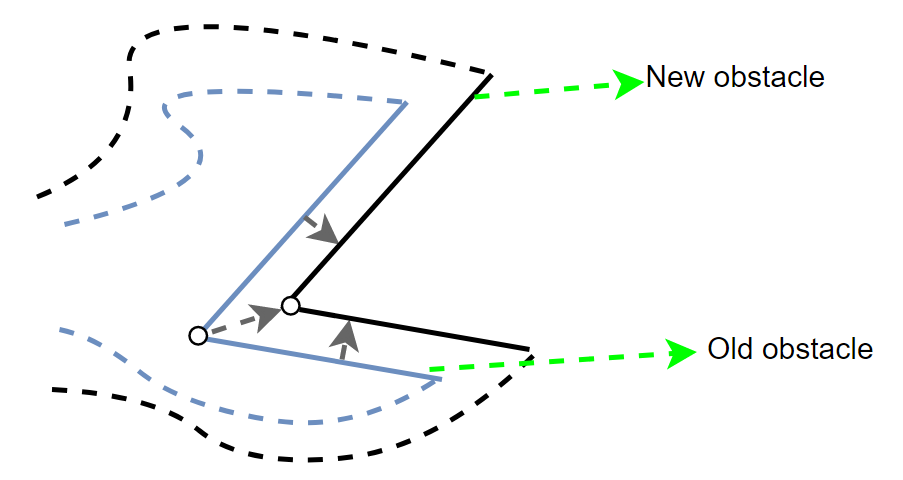
\includegraphics[width=0.7\textwidth]{Robot_Global_Vision_Update/RGVU_fconfig_lom.png}
							\caption{Jordan Curve Theorem}
						\end{figure} \\
						\item[$\circ$] If 2 edges form a convex vertex, then the algorithm will find normal vectors move the edges like the same with case 1 above. After that, it find an bisector of the vertex in the direction out of the obstacle, the length of bisector is equal to robot radius.\\
						The bisector is calculated based on vector of 2 edges. This is the reason we need to process the three adjacent collinear points before using the obstacles zooming-in algorithm. If there are 3 adjacent collinear points, then the normal vector of the 2 sides and the bisector have the same direction, so it is impossible to find the intersection between them.\\
						Finally, it calculate intersection points of 2 edges with a line perpendicular to the bisector which has distance of robot radius from the old vertex. The old vertex will be replaced by 2 intersection points calculated.\\
						
						\begin{figure}[!h]
							\centering                                 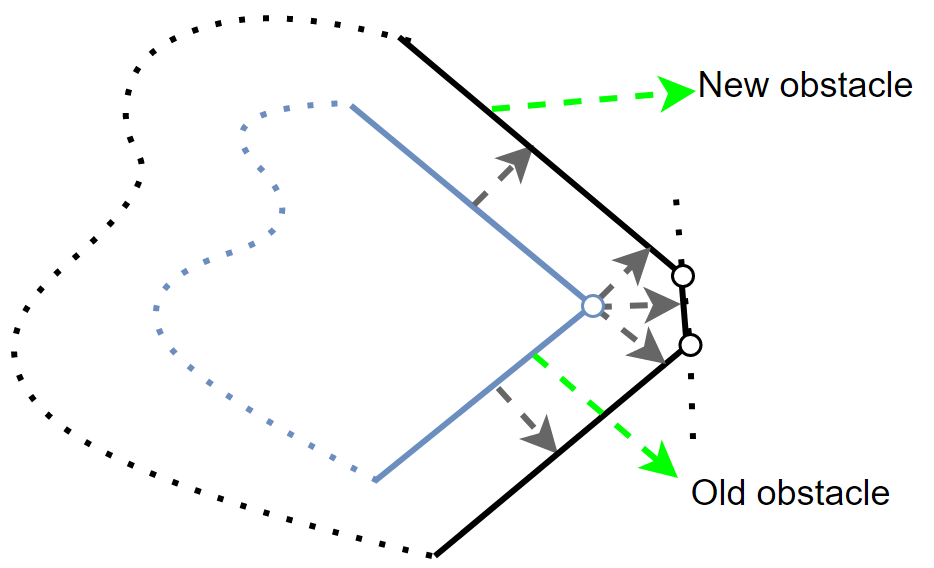
\includegraphics[width=0.7\textwidth]{Robot_Global_Vision_Update/RGVU_fconfig_loi.png}
							\caption{Jordan Curve Theorem}
						\end{figure} \\
					\end{itemize}
				
					After traversing all pairs of adjacent edges, the algorithm return an obstacles list that contain obstacles after zooming-in as the figure below. \\
					\begin{figure}[!h]
						\centering                                 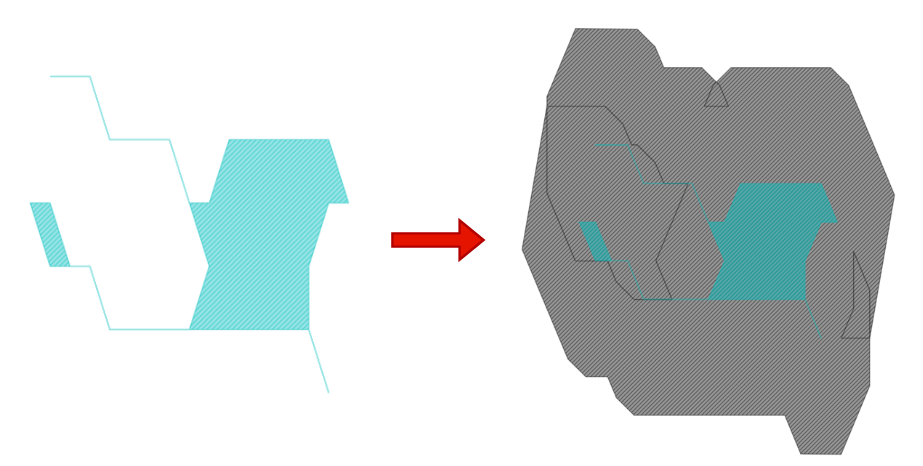
\includegraphics[width=0.7\textwidth]{Robot_Global_Vision_Update/RGVU_fconfig_result.png}
						\caption{Jordan Curve Theorem}
					\end{figure} \\
					
				\end{itemize}
				As we see the obstacle after zooming-in, there exists the wrong edge insde obstacle. Therefore, to ensure that the algorithm for finding open sight and open points works as expected, the obstacle needs to go through a post-processing step to remove the vertices inside the obstacles.
				
				\item[$\ast$] \textbf{Obstacles post-processing algorithm}
				\textit{Obstacles post-processing algorithm} is used to remove any edge inside obstacle.\\
				The open sights and open points finding algorithm applied in case obstacle is correct polygon (as described in \textit{Three collinear adjacent vertices removing} algorithm). As we saw the result after obstacle zooming-in step, the obstacle exists edges and vertices inside it. The cause of this one is that the obstacle actually has a lot of edges close together, so when applying the zooming-in algorithm, edges after zooming will intersect inside the new obstacle, thereby leading to the formation of vertices and edges inside it.\\
				\begin{figure}[!h]
					\centering                                 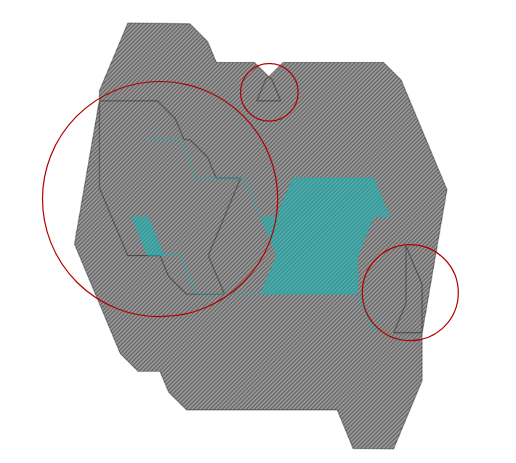
\includegraphics[width=0.7\textwidth]{Robot_Global_Vision_Update/RGVU_zoom-in_error.png}
					\caption{Zoomed-in obstacle has edges and vertices inside}
				\end{figure} \\
				This algorithm is implemented based on finding an edge whose vertex lies inside the obstacle. If it exists, the algorithm will drop all subsequent vertices until it finds an edge whose vertex lies outside the obstacle. \\
				\begin{figure}[!h]
					\centering                                 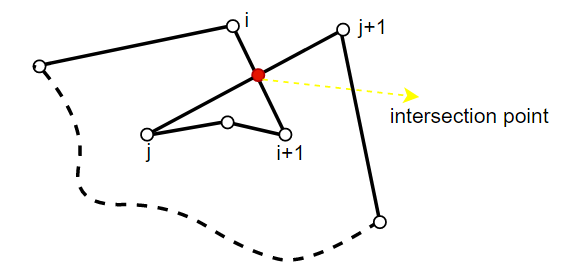
\includegraphics[width=0.7\textwidth]{Robot_Global_Vision_Update/RGVU_posprocess.png}
					\caption{\textit{Obstacles Pos-processing} algorithm}
				\end{figure} \\
				The algorithm keep one edge has index $i:i+1$ of the obstacle and traverse all remaining edges afterwards in list (which has index bigger than $i+1$). If it found an edge index $j:j+1$ which intersects an edge keeped, it would pop all point from $i+1$ to $j$ and append new vertex is an intersection point of 2 edges under review. The process repeats for all edges in the obstacle.\\
				\begin{figure}[!h]
					\centering                                 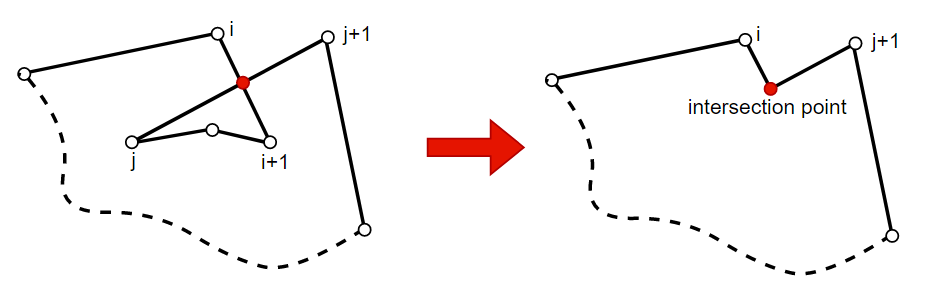
\includegraphics[width=0.7\textwidth]{Robot_Global_Vision_Update/RGVU_posprocess_before_after_pop.png}
					\caption{\textit{Obstacles Pos-processing} algorithm}
				\end{figure} \\
				After applied algorithm, the zoomed-in obstacles will no longer have vertices inside it. This will ensure the open points finding algorithm works as the theory and finds safe openings for robot movement.
				\begin{figure}[!h]
					\centering                                 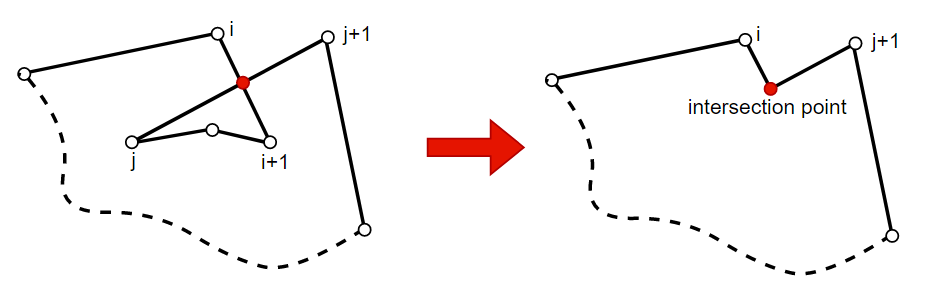
\includegraphics[width=0.7\textwidth]{Robot_Global_Vision_Update/RGVU_posprocess_before_after_pop.png}
					\caption{Obstacles before and after using \textit{Obstacles Pos-processing} algorithm}
				\end{figure} \\
			\end{itemize}
		
			
	
\end{document}